% Drawing 156-4/03-5 -- folder 156-4, batch 03, archive page 51 (PDF page 52).
% Transcription: moitié gauche, en bas, entouré d'un grand arc, un cube de relations : en haut $\Phi \subset \overline{F}'$, $\widetilde{F}$, $\vec{F}$, $F$ ; au milieu $F'$ ; en bas $\overline{G}'$, $\widetilde{G}$, $\overline{G}$, $G$, $G'$ ; des flèches marquées $\simeq$ (subdivisions) et des flèches verticales.
% Kind: cube of relations (large arrow diagram). Method 2 (schematic redraw from the facsimile). Status: partial.
% Notes: Large arrow diagram, drawn as the skill prescribes for these: nodes placed as on the page, the principal arrows between them, labels as the transcription reads them. Top face: Phi (included in) -> F-bar'; F-bar' to F-tilde by a curved inclusion arrow; F-tilde ~-> F-vec ~-> F. Middle: F', reached from F-bar' by a ~-> arrow and joined to F-vec by a curved inclusion arrow; a vertical stroke from F-tilde down to F'. Bottom face: G-bar', G-tilde ~-> G-bar ~-> G, and G' reached from G-bar' by a ~-> arrow, with a short inclusion hook from G' towards G-bar and from G-bar' towards G-tilde. Vertical strokes: F-bar' down to G-bar', F' down to G-tilde, F-vec down to G-bar, F down to G, and a long vertical from F' down past G-tilde to G'. The large arc that encloses it is drawn. Left out: the heavy hatched scribble at the top (struck), and the F' at the far left joined to it by a double stroke (read as part of that struck insertion; doubtful). Arrowheads and hooks are approximate. Method: a relation diagram of formulas, which the transcription skill would set as text (tikz-cd); since it stands only as a \drawing mark, it is set here as a TikZ layout of the formula: every symbol is a LaTeX text node at its place on the page, the arrows are drawn between them. Redrawn 2026-11-09 (issue 128): to check again. Question settled by a machine pass on the facsimile, 2026-11-12 (maths): the F' at the far left is crossed by the same double stroke that leads into the hatched scribble, and no arrow of the cube reaches it; the cube needs one F' only, the middle one, which carries the arrows from F-bar' and to F-vec. The far-left F' is struck with the insertion and stays left out. Not checked by a reader.
% Coordinates: 1 unit = 1 mm = 1/100 of the crop width (bbox in page fractions: [0.06, 0.7, 0.46, 0.9]).
% Redrawn by Claude (claude-opus-5-5), issue #73, 2026-11-09; not checked by a human; not compiled (no TeX in the session).
% Rights: reproduces part of the work -- behind RENDER_TRANSCRIPTS, never published by itself.
\documentclass[tikz,border=3pt]{standalone}
\usepackage{amsmath,amssymb}
\usetikzlibrary{patterns,arrows.meta}
\tikzset{pencil/.style={black!45}, struck/.style={black!35}, mark/.style={circle,draw,inner sep=1.3pt}, pt/.style={circle,fill,inner sep=0.9pt}, opt/.style={circle,draw,fill=white,inner sep=1.1pt}}
\begin{document}
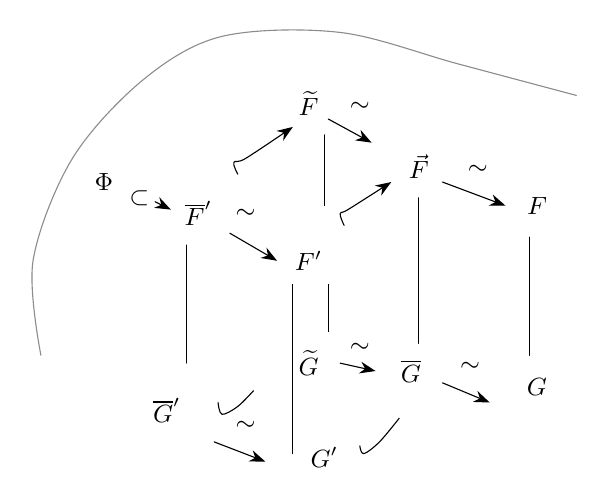
\begin{tikzpicture}[x=1mm,y=1mm,line cap=round,line join=round,font=\scriptsize]
\draw[pencil] plot[smooth, tension=0.55] coordinates {(32,-45) (31,-33) (36,-20) (45,-10) (55,-4.5) (70,-4) (85,-8) (100,-12)};
\node[inner sep=1pt] at (40,-23) {\small $\Phi$};
\node[inner sep=1pt] at (44.5,-25) {\small $\subset$};
\draw[-{Stealth[length=2mm]}] (46.5,-25.5) -- (48.5,-26.5);
\node[inner sep=1pt] at (52,-27) {\small $\overline{F}'$};
\node[inner sep=1pt] at (66,-13) {\small $\widetilde{F}$};
\node[inner sep=1pt] at (80,-21) {\small $\vec{F}$};
\node[inner sep=1pt] at (95,-26) {\small $F$};
\node[inner sep=1pt] at (66,-33) {\small $F'$};
\draw[-{Stealth[length=2mm]}] plot[smooth, tension=0.55] coordinates {(57,-22) (56.5,-20.5) (58,-20) (64,-16)};
\draw[-{Stealth[length=2mm]}] (68.5,-15) -- (74,-18);
\node[inner sep=1pt] at (72.5,-13.5) {\small $\sim$};
\draw[-{Stealth[length=2mm]}] (83,-23) -- (91,-26);
\node[inner sep=1pt] at (87.5,-21.5) {\small $\sim$};
\draw[-{Stealth[length=2mm]}] (56,-29.5) -- (62,-33);
\node[inner sep=1pt] at (58,-27) {\small $\sim$};
\draw[-{Stealth[length=2mm]}] plot[smooth, tension=0.55] coordinates {(70.5,-28.5) (70,-27) (71,-26.5) (76.5,-23)};
\draw (68,-17) -- (68,-26);
\draw (50.5,-31) -- (50.5,-46);
\draw (68.5,-36) -- (68.5,-42);
\draw (80,-25) -- (80,-43.5);
\draw (94,-30) -- (94,-45);
\draw (64,-36) -- (64,-57.5);
\node[inner sep=1pt] at (48,-52) {\small $\overline{G}'$};
\node[inner sep=1pt] at (66,-46) {\small $\widetilde{G}$};
\node[inner sep=1pt] at (79,-47) {\small $\overline{G}$};
\node[inner sep=1pt] at (95,-49) {\small $G$};
\node[inner sep=1pt] at (68,-58) {\small $G'$};
\draw[-{Stealth[length=2mm]}] (70,-46) -- (74.5,-47);
\node[inner sep=1pt] at (72.5,-44) {\small $\sim$};
\draw[-{Stealth[length=2mm]}] (83,-48.5) -- (89,-51);
\node[inner sep=1pt] at (86.5,-46.5) {\small $\sim$};
\draw[-{Stealth[length=2mm]}] (54,-56) -- (60.5,-58.5);
\node[inner sep=1pt] at (58,-54) {\small $\sim$};
\draw plot[smooth, tension=0.55] coordinates {(54.5,-51) (55,-52.5) (57,-51.5) (59,-49.5)};
\draw plot[smooth, tension=0.55] coordinates {(72.5,-56.5) (73,-57.5) (75,-56) (77.5,-53)};
\end{tikzpicture}
\end{document}
